% !TEX encoding = UTF-8 Unicode
% !TEX root = thesis.tex
% !TEX spellcheck = en-US
%%=========================================
\chapter[Social Media Attacks]{Social Media attacks on mobile devices vs. attacks on computers}
\section{Management summary}
\subsection*{Topic}
In this paper I am looking at the differences between the security topography for social media users, on a mobile device, versus that one face when using a personal computer.
\subsection*{Intro}
We have seen an enormous increase in online social media in popularity during the past decade. It has taken over a lot of the networking people tended to do in real life earlier and it makes keeping in touch with a larger network of people a less laboursome task. We tend to trust a friend more than we would any random person on the street and this trust mechanism has been transferred to the cyber space.
\subsection*{The threat picture}
I have found quite a few differences and in other areas the situation is quite similar. The conclusion I reached was that it is, at least at present, much safer to use social media on a regular personal computer than on a mobile device, but that it also depends to a great degree how the user behaves security vice. The share of time people spends on social media networks on their mobile device, versus on their computer, is according to comScore already 79\% vs 21\% and still the mobile platform is rapidly gaining terrain. The mobile platforms are getting better protection, but still they are behind on sophistication level when it comes to security. From what I have seen it looks as if you are an easier target for social media attacks when you are using a mobile device, than you are doing the same social media networking on your computer.
\subsection*{How to have a measure of security while still utilizing the potential}
So how do we make sure we are able to maximize the profit from both the mobility and BYOD-trends in the workplace, the increased social network our employees get access to when using social media and last but not least the large, but not so easily calculated, branding value for our business by having a strong presence in social media?
We have to make sure we profit from the positive side of the risk, or opportunity if you want, while at the same time making sure that we have a reasonably secure mobile infrastructure in place. It will never be a good option to withdraw from the use of social media on mobile devices, we would simply lose too much terrain to the competition.
The easiest and most commonplace solution to this problem in the industry today. is to implement an MDMS, a Mobile Device Management System. This will ensure that we can encrypt the work related content on the devices and keep it separated from the personal content the users have. This gives us the opportunity to remotely erase data when devices are lost or stolen

\section{Abstract}
We have seen an enormous increase in online social media in popularity during the past decade. It has taken over a lot of the networking people tended to do in real life earlier and it makes keeping in touch with a larger network of people a less laboursome task. We tend to trust a friend more than we would any random person on the street and this trust mechanism has been transferred to the cyber space. Cybercriminals, who seem to be mostly concerned with gaining wealth, political high ground, or are ideologically motivated, have shown a keen interest in utilizing these new networking platforms. They come from several different directions, such as attacking via vulnerabilities in hardware, OS, protocols, and apps, but they are also successfully exploiting the trust that exists between members of a social network.
In this paper I am looking at the differences between the security topography for social media users, on a mobile device, versus that one faced when using a personal computer. I have found quite a few differences and in other areas the situation is quite similar. The conclusion I reached was that it is, at least at present, much safer to use social media on a regular personal computer than on a mobile device, but that it also depends to a great degree how the user behaves security vice. The share of time people spend on social media networks on their mobile device versus on their computer is already 79\% vs 21\% [11] and still the mobile platform is rapidly gaining terrain. The mobile platforms are getting better protection, but still they are behind on sophistication level when it comes to security. From what I have seen it looks as if you are an easier target for social media attacks when you are using a mobile device than you are doing the same social media networking on your computer.

\section{Hypothesis and methodology}
My hypothesis is that it is easier to attack social media users via their mobile platform gadgets, than via their use of the same media on computers. I have weighed different factors and gathered information around the subject by reading published material saying something about usage pattern, platform weaknesses, distribution of vulnerabilities, and how the users time is divided between the two platform categories. I have looked at how software and hardware protection is being utilized the two cases and I will in the end try to conclude based upon the information presented.
 The subject of social has been moving so quickly, behavioural statistics changing drastically from one year to the next. This constant change makes it difficult to obtain standard peer reviewed research with the latest numbers. For this reason, I have partially leaned on numbers obtained from white papers published by some of the big commercial players in the information security market. These papers are recognized by the industry as reliable sources for such information.
\section{Introduction}
Social media attacks are increasingly common. People’s usage pattern of social media has also changed dramatically during the past few years. An increasing amount of people’s social media interaction is being conducted on mobile hardware platforms. Instead of using Facebook, LinkedIn and other media on the Personal Computer they may or may not still have in their home, they are now using the same media on their mobile devices, such as pads and smartphones. There are also new social media appearing, especially made for these mobile platforms, such as Instagram, which is made to share photos taken with your smartphone on the go.
People now spend more time interacting on social media using their smartphone, than they do using their computer. According to comScore 79\% vs 21\% \cite{CrossPlatform2016}. Since this is a relatively new trend, that has exploded in the past couple of years, it is interesting to see if the migration from one platform to another has led to a more unsecure situation for the users. I limit the type of attack here to direct attacks on end users, with the intension to extract either labour, money or personal data. Nevertheless, I think that the result says something about the security difference we currently have between these two types of platforms.
\section{Attacks on social media users in general}
Some of the most popular social media providers today are Facebook, LinkedIn, Twitter, Google+, YouTube, Pinterest, Instagram, Vine, Snapchat and Reddit. There are myriads more and new services pop up all the time.
While using portable devices to access social media, the user is both a possible target for the same types of attacks that we find being used against computer users and at the same time the limited resources of the mobile devices limits the possibility of using the same advanced mechanisms and software to stay safe \cite{Zonouz2013215}.
Most attacks on the users of these media are economically motivated. There can be different paths to earning money on a social media attack. The reason for an attack can also be politically motivated or even nation state security concerns. I’ll go through a few and compare possibilities on the different platforms.
As the mobile devices gets ever more advanced and the number of apps, protocols and uses seem to rise towards the sky, it is no big surprise that the number of vulnerabilities follows suit as seen in Figure \ref{fig:mobile_vulnerabilities}.
\begin{figure}
\centering
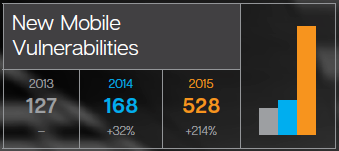
\includegraphics[width=0.5 \textwidth]{fig/mobile_vulnerabilities}
\caption{New mobile device vulnerabilities per year \cite{ISTR2016}.\label{fig:mobile_vulnerabilities}}
\end{figure}
\section{Specific attack vectors for computers}
Microsoft Windows has been the most widely used operating system and thereby represent the largest attackable population. It has also been regarded much easier to attack than the other common computer operating systems, because of the way it is built. 
Apples operating system was long regarded as the safest choice of operating system for a computer, but in the past couple of years there has been discovered many new vulnerabilities and also attack vectors that does not need vulnerabilities to be executed. The fact that this operating system is much less popular than MS Windows also makes it less attractive for an attacker, unless it is directed against a community where Apple products are the most common chiose.
\section{Specific attack vectors for smartphones}
\subsubsection{Android}
New types of attacks are coming all the time. Cross platform attack on Android is being performed via Google Play in a web browser on an ordinary computer. When the victim logs on to the Google Play account on a computer, to install apps on a mobile device running Android, malware on the computer can steal the browser cookies for that session and use it to impersonate the user. It is then possible for the attacker to remotely install apps on the victim’s Android unit. We can also see that the malware is becoming smarter and the sophistication level is rapidly reaching the level of malware for computers. Example are that they are now both obfuscating the code so as not to be detected by malware protection software that uses signatures, and malware that can check if it is running on a real device or a security company’s emulator, thereby avoiding detection. Another weakness with the Android platform is that even if Google pushes out security patches to the makers of all the different devices as fast as they can, many makers take a long time to push these out to their end users \cite{ISTR2016}.
\subsection{iOS}
Apples screening of apps, before letting them into their App store, is very strict, so one can generally be more trusting towards apps found there. Attackers of Apple’s portable devices, running the iOS operating system, for the most had to rely on finding vulnerabilities or attack a jailbroken device to succeed (unlike Android). This is no longer the case. Several new ways of attacking these devices has recently come to light. Symantec mentions two examples of such attack techniques namely XcodeGhost and YiSpectre which can compromise an iOS device without using vulnerabilities or jailbreaking.
\begin{figure}
\centering
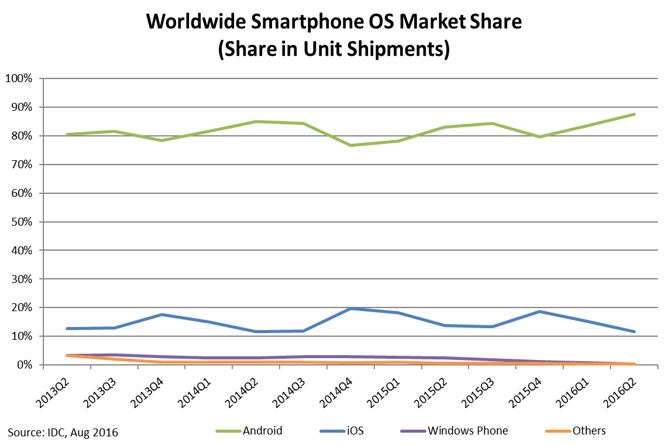
\includegraphics[width=0.8 \textwidth]{fig/smartphone_market_share}
\caption{According to IDC (IDC, Aug 2016) the market share for the Android smartphone OS in August 2016 was 87.6\% And for iOS 11.7\%.\label{fig:smartphone_market_share}}
\end{figure}
The OS distribution in the market means that attackers probably concentrate on Android to get the highest return for their effort. In fact, Kaspersky Lab and INTERPOL has made a report that states that an estimated 98.05\% of all malware is coded to target Android. They also found (in 2014) that the number of detected malware programs for Android had almost tripled since the previous year \cite{Kaspersky2014}. 
\section{Social media attacks directly on the given platform}
As we have seen there are many ways of attacking social media users/accounts via the platform they are using the media on. There are however a lot of ways to attack via the social media itself, without depending on vulnerabilities in the hardware or software. The attacks simply rely on the many vulnerabilities found in the users, so to speak. These kind of attacks are usually categorized as 
\subsection{User behavioural aspects}
\subsection{Hardware and software}
The way we use these mobile platforms will largely effect how safe we are from attacks. A lot depends on whether the user installs some kind of antivirus/antimalware program on their device and also how the user thinks about security, compare to when using computer.
Many users leave the Wi-Fi on all the time. It is convenient to have your device connect automatically to all the networks you use, but this convenience comes at a high cost security wise. It is increasingly easy to attack these users by setting up a portable “Wi-Fi-box” that answers the unknowing smartphone owner’s device’s call for a named network, saying “Yes, here I am, please connect to me”. Such devices can be bought readymade on the Internet; an example is the Wi-Fi Pineapple (https://www.wifipineapple.com/).
The other radios in the devices, like Bluetooth and NFC, are also possible entry points for an attacker. We have seen attacks lately using NFC-code stickers containing malicious code or pointing the device user to a malicious website. These stickers can be bought for less than a dollar, programmed via a smartphone and printed with for example “Scan to get 100 free Instagram followers” or something to get people to scan it. An example of a possible attack could be to make the sticker point the user to a mock-up web page that looks like Instagram and since they already think they are there to get more followers they wouldn’t react on having to enter their username and password. 
\subsection{Social media network trust}
People build their social networks online, for most, as they do in real life. They either do know or at least feel they know the people in their social media network to a certain extent. This again leads to trust. People tend to trust the people in their social media network, just the way they trust their friends and co-workers’ in real life.
This trust makes the users easy prey to attackers making it look like links and other things has been sent to them by someone in their network. This can be both sent directly as a personal message, shared to all friends or simply liked. The most popular form of social media scam is manual sharing. Manual sharing consists of something that looks great in some way so that users themselves will want to share it with their friends, like for example a cool video or the chance of winning a new car if you share the post.
\begin{figure}
\centering
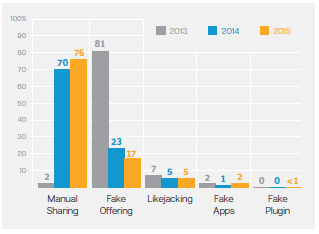
\includegraphics[width=0.5 \textwidth]{fig/social_media_scams}
\caption{Social media network scams by popularity \cite{ISTR2016}.\label{fig:social_media_scams}}
\end{figure}
The mechanisms of these scams works the same regardless of platform, since they are relying on the intended functionality of the app or web page. There should not be any difference in the way people
\section{Conclusion}
Based upon the material I have reviewed I would have to conclude that it is much easier to attack social media users via their portable devices, than it would be to attack their computer. The main considerations behind my conclusion are the following: The majority of time spent on social media is spent accessing these on a mobile device and not a computer. Very few people install any form of malware protection on their mobile devices, while a good majority installs malware protection on their computers. The malware protection solutions that exists for mobile devices, are inferior to the systems available to do the same task on a computer. The number of vulnerabilities found for mobile devices per year is rising quickly. People tend to walk around town with Wi-Fi, Bluetooth, and NFC turned on for anyone to exploit.
So the advice to the general public should be to at least install some sort of malware protection on all their devices, don’t leave Wi-Fi, Bluetooth or NFC on when it is not in use.
\section{Grade argument}
To argue for my own grade is new to me, it feels kind of intimidating for a Norwegian to do this but I’ll give it a try.
We have been working on this task for most of the semester and it has given me some sorely needed writing experience. I often find it difficult to write enough, length wise in the tasks given, because I am prone to go straight for the point rather than discuss, weigh it, and look at it from different angles.
Never the less, here we are at the end of the semester and I think I have done a pretty good job. To place it on a scale from “A” to “F” is not easy, but let’s start out at the top and see what would subtract from that.
To get an “A” I believe there should have been more details and probably there is also room for giving the terminology of the course material a more prominent place in the text. I found it rather difficult to limit the task properly, but I have certainly given it my best shot. 
On the other side, I feel I have succeeded in presenting the material in an easy and not too technical manner, so that it would be easily understood by the board of a company, should they wish to read not only the executive summary, but the entire chapter. I also think the language is pretty good and should not present an obstacle to the reader.
Based on these pros and cons I would give myself a “B”
